\section{Systems with known instability problems}
\graphicspath{{figures/"Preanalysis&Requirement"/SimilarSystems/}}
In order to stabilize the rocket in flight, a controller must be designed to stabilize the vertical position during flight.The possibility of damaging the rocket or the controller needs to be countered by the efficiency of the control system. Experimenting such a system during flight is expensive and presents nonnegligible hazards.
Is there a system that has similar instability properties of rockets, and presents fewer restrictions to experiment?

An inverted pendulum objective is to stabilize a stick whose center of mass is above pivot point. The process is done using a horizontal force, resulting in a first degree of freedom rotation, as found in a rocket system. An example of an inverted pendulum would be humans. Adjustments are needed to maintain balance when standing, walking, or running. 
A double inverted pendulum is a combination of an inverted pendulum and a double pendulum. The stability of the stick is reached by appliying a torque between the two pendulums.To reach the equilibrium position of a rocket in flight, the aileron must create a torque to counter the lift force. Flight are not required to experiment the system, therefore it is less restrictive to use and analyze an inverted pendulum or double inverted pendulum. 

\begin{figure}[htbp]
	\centering
	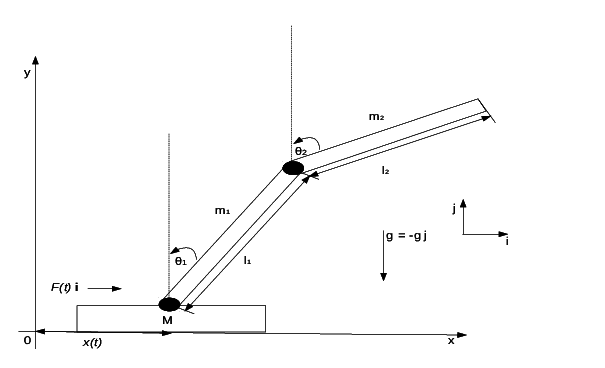
\includegraphics[width=0.6\linewidth]{double-inverted-pendulum}
	\caption{Summary of forces applied to a double inverted pendulum. The process is equivalent to figure  \vref{fig:RocketForceSummary}.}
	\label{fig:InvertedPendulum}
\end{figure}



The Cubli is another system known for its instability. It is commonly used in Control Theory to analyze the behavior of a reaction of a wheel inverted system. The advantages of the usage a Cubli is its ability to reach its equilibrium position in microgravity environments, such as asteroids. This is not relevant to a rocket instability project.

A recent technology facing instability is Segway. A Segway is an application of an inverted pendulum to a two wheeled self-balance vehicle. The objective is to detect and stabilize the instability of the vertical stick to move the vehicle and prevent the user to fall.vehicle when moving in order This vehicle requires three body directions instead of the linear motion of an inverted pendulum. The study of instability properties of a Segway system would mean the study of elements nonexistent or negligible in a rocket system.

In consideration of the different applications and similarities of the three systems, the double inverted pendulum will be analyzed to develop a model describing the dynamics of the system, and to design a control system stabilizing the position in vertical position. The objective is to understand and solve the instability properties shared by rocket and inverted pendulum systems.

